\chapter{دوال الموجة للمذبذب، واللفّ المغزلي نصفي، وتبادل الجسيمات}

\section{المذبذبات في كل مكان}

يمكن لأي نظام له اتزان مستقر أن يتذبذب عندما يُزاح عن ذلك الاتزان. وقد يكون له تردد واحد أو عدة ترددات. فوتر الكمان، على سبيل المثال، له نمط أساسي وتوافقيات أعلى. ونقره يثير تركيبًا ما من تلك الأنماط.

غير أن الأمثلة الأهم هنا هي الحقول. فتهيئة الاتزان للحقل الكهرومغناطيسي هي الفراغ: لا مجال كهربائي، ولا مجال مغناطيسي، ولا تذبذب كهرومغناطيسي. وإذا أُدخل إشعاع إلى تجويف أو إلى دليل موجي، أمكن للحقل أن يتذبذب في أنماطه المسموح بها، ولكل منها ترددها الخاص. وفي النظرية الكمية تصف تلك الأنماط مجموعات من الفوتونات.

وتنطبق الفكرة نفسها على البلورة. ومن المضلل أن نتصور كل ذرة على أنها مذبذب مستقل. فالذرات تؤثر بعضها في بعض بقوى، لذا فإن إزاحة ذرة واحدة تؤثر في جاراتها وتنتقل موجة عبر البلورة. والأنماط العادية لتلك الحركة المقترنة هي مذبذبات توافقية، وتسمى كمّاتها فونونات. والفوتونات والفونونات أشياء فيزيائية مختلفة، لكن كليهما يعيدنا إلى جبر المذبذب نفسه.

\section{جبر المذبذب}

في مناقشة المذبذب، نأخذ الكتلة وثابت بلانك المختزل مساويين للواحد:
\[
m=1,\qquad \hbar=1.
\]
ويكون الهاملتوني
\begin{equation}
H=\frac{p^{2}}{2}+\frac{\omega^{2}x^{2}}{2}.
\end{equation}
ويحدد المعامل \(\omega\) انحناء الجهد، وهو أيضًا تردد التذبذب.

عرّف مؤثري الرفع والخفض بـ
\begin{equation}
A_{\pm}=\frac{p\pm i\omega x}{\sqrt{2\omega}}.
\end{equation}
واختير عامل التطبيع بحيث
\begin{equation}
[A_{-},A_{+}]=1.
\end{equation}
ومؤثر العدد هو
\begin{equation}
N=A_{+}A_{-}.
\end{equation}
ومعًا، تفيد هذه المعادلات أن \(A_{+}\) يرفع قيمة ذاتية لـ \(N\) بمقدار واحد، وأن \(A_{-}\) يخفضها بمقدار واحد. والطيف الناتج هو
\begin{equation}
n=0,1,2,3,\ldots .
\end{equation}

كما أن ضرب مؤثري السُّلَّم أحدهما في الآخر يكشف التصحيح الكمي للطاقة الكلاسيكية:
\begin{align}
N
&=\frac{1}{2\omega}(p+i\omega x)(p-i\omega x)\\
&=\frac{1}{2\omega}\left(p^{2}+\omega^{2}x^{2}
 +i\omega[x,p]\right)\\
&=\frac{1}{2\omega}\left(p^{2}+\omega^{2}x^{2}-\omega\right),
\end{align}
حيث \([x,p]=i\). وبالتالي،
\begin{equation}
H=\omega\left(N+\frac12\right).
\end{equation}
وإذا كان الثابت الإضافي غير ذي صلة بالمسألة، فمن الملائم استعمال الهاملتوني المزاح
\begin{equation}
H_{\mathrm{shifted}}=H-\frac{\omega}{2}=\omega N.
\end{equation}
والحد \(\omega/2\) هو طاقة النقطة الصفرية، أو طاقة الحالة الأرضية، للمذبذب. وبالنسبة إلى نمط حقلي، يسمى الحد المناظر طاقة الفراغ. وهو يعكس مبدأ عدم اليقين: فلا يمكن لأي حالة أن يكون فيها كل من \(x\) و\(p\) مساويًا للصفر على نحو حاد، ولذلك لا يمكن أن تكون للحدين التربيعيين الموجبين في \(H\) قيمة توقعية صفرية معًا.

\begin{classroomqa}
\lecturetimestamp{00:09:46}
\audiencequestion{لماذا يشتمل طيف مؤثر العدد على الصفر؟}
\lecturerresponse{يمكن البرهنة على ذلك صراحةً ببناء الدالة الموجية للحالة الأرضية. وسيُظهر هذا البناء حالةً لها \(N=0\).}
\end{classroomqa}

ولبدء هذا البناء، استبدل متجهات الحالة بدوال موجية للموضع. فتصبح حالات الطاقة الذاتية
\[
\psi_{0}(x),\ \psi_{1}(x),\ \psi_{2}(x),\ldots,
\]
وتؤثر المؤثرات الأساسية على النحو
\begin{equation}
X\longmapsto x,\qquad
P\longmapsto -i\frac{d}{dx}.
\end{equation}
ومع إعادة \(\hbar\)، يصبح الاستبدال الثاني
\(P\mapsto-i\hbar\,d/dx\).

قبل حل \(\psi_{0}\)، توجد إجابة تجريدية أسرع عن السؤال. فعلى سُلَّم حالات القيم الذاتية المنفصل والقابلة للتطبيع للمذبذب، يكون \(N=A_{+}A_{-}\) غير سالب، لذا لا يمكن أن يستمر الخفض المتكرر بخطوات وحدوية إلى ما لا نهاية. وعند الطرف النهائي---الذي ستُبنى دالته الموجية القابلة للتطبيع أدناه---لا بد من وجود حالة، نرمز لها بـ \(\lvert0\rangle\)، بحيث
\begin{equation}
A_{-}\lvert0\rangle=\mathbf 0.
\end{equation}
وإلا لكان \(A_{-}\lvert0\rangle\) حالةً أخرى أخفض بدرجة واحدة. ويترتب على ذلك فورًا أن
\begin{equation}
N\lvert0\rangle
=A_{+}A_{-}\lvert0\rangle
=\mathbf 0
=0\,\lvert0\rangle.
\end{equation}
ومن ثم فإن القيمة الذاتية لمؤثر العدد في الحالة الدنيا هي الصفر.

\begin{classroomqa}
\lecturetimestamp{00:14:57}
\audiencequestion{إذا كانت القيمة الذاتية هي الصفر، أفلا ينبغي أن يحتوي الطرف الأيمن على متجه ذاتي صفري؟}
\lecturerresponse{الكت \(\lvert0\rangle\) متجه مطبَّع غير صفري ووسمه صفر. وفي \(N\lvert0\rangle=0\,\lvert0\rangle\) يكون الطرف الأيمن هو المتجه الصفري. وكت الحالة الأرضية والمتجه الصفري شيئان مختلفان.}
\end{classroomqa}

\section{معادلة Schr\"odinger والحلول الفيزيائية}

لنعد الآن إلى تمثيل الموضع. معادلة Schr\"odinger غير المعتمدة على الزمن هي
\begin{equation}
\left[
-\frac12\frac{d^{2}}{dx^{2}}
+\frac12\omega^{2}x^{2}
\right]\psi(x)=E\psi(x).
\end{equation}
وبوصفها معادلة تفاضلية من الرتبة الثانية، فلها حلول صورية لقيم اعتباطية لـ \(E\). وليست معظم تلك الحلول الصورية حالات فيزيائية للمذبذب. إذ إنها تنمو أسيًا عند القيم الكبيرة لـ \(\lvert x\rvert\)، ولذلك يتباعد معيارها.

في الحالة المقيدة، يجب أن تكون الدالة الموجية قابلة للتكامل تربيعيًا:
\begin{equation}
\int_{-\infty}^{\infty}\psi^{*}(x)\psi(x)\,dx<\infty.
\end{equation}
وعندئذ يمكن تطبيعها بحيث يساوي التكامل واحدًا. ولا تنتج مثل هذه الحلول إلا عن قيم خاصة للطاقة. وحالات الموضع والزخم على مستقيم لا نهائي استثنائية من هذه الناحية، لكن حلول المذبذب التي تنمو أسيًا تُستبعد ببساطة من فضاء الحالات.

\section{الحالة الأرضية الغاوسية}

يمكن حل معادلة الرتبة الثانية، لكن جبر السُّلَّم يعطينا معادلة أبسط من الرتبة الأولى:
\begin{equation}
A_{-}\psi_{0}(x)=0.
\end{equation}
والعامل الكلي في \(A_{-}\) غير مؤثر عندما يكون الطرف الأيمن صفرًا، ولذلك يكافئ هذا
\begin{equation}
(p-i\omega x)\psi_{0}(x)=0.
\end{equation}
وباستخدام \(p=-i\,d/dx\) نحصل على
\begin{equation}
\left(\frac{d}{dx}+\omega x\right)\psi_{0}(x)=0.
\end{equation}

\begin{classroomqa}
\lecturetimestamp{00:22:32}
\audiencequestion{هل يمكن حل هذا بفصل المتغيرات؟}
\lecturerresponse{ليس هناك إلا متغير مستقل واحد، لذلك لا يوجد متغيران لفصلهما. وعند كتابة المعادلة على الصورة \(\psi_{0}'/\psi_{0}=-\omega x\)، تكون على هيئة مشتقة لوغاريتمية. وهذا يقترح كتابة الدالة الموجية على هيئة أسية.}
\end{classroomqa}

ومن الطرق المفيدة لحلها أن نكتب
\begin{equation}
\psi_{0}(x)=e^{f(x)}.
\end{equation}
وعندئذ
\[
\psi_{0}'(x)=f'(x)e^{f(x)},
\]
ويلغى العامل الأسي المشترك. وتختزل المعادلة إلى
\begin{equation}
\frac{df}{dx}+\omega x=0.
\end{equation}

\begin{classroomqa}
\lecturetimestamp{00:26:28}
\audiencequestion{هل ينبغي أن تظهر إشارة سالب في \(f(x)\)؟}
\lecturerresponse{نعم. بما أن \(df/dx=-\omega x\)، فإن التكامل يعطي حدًا تربيعيًا سالبًا.}
\end{classroomqa}

إذن
\begin{equation}
f(x)=-\frac12\omega x^{2}+C,
\end{equation}
و
\begin{equation}
\psi_{0}(x)\propto e^{-\omega x^{2}/2}.
\end{equation}
ويُترك ثابت التطبيع الضربي دون تحديد. والنقطة المهمة هي الشكل الغاوسي: فهو أملس، ومتمركز قرب الأصل، ويتناقص سريعًا عند القيم الكبيرة لـ \(\lvert x\rvert\). ومن الواضح أنه قابل للتكامل تربيعيًا.

لا حاجة إلى إعادة التعويض بالحل في معادلة الرتبة الثانية لاستخراج طاقته. فالجبر يعطينا بالفعل
\begin{equation}
E_{0}=\frac{\omega}{2}.
\end{equation}

\section{الحالات المثارة، والعقد، والحركة الكلاسيكية}

تنتج الحالة المثارة الأولى من رفع الحالة الأرضية:
\begin{equation}
\psi_{1}(x)\propto A_{+}\psi_{0}(x)
\propto(p+i\omega x)e^{-\omega x^{2}/2}.
\end{equation}
ومعادلة الحالة الأرضية تقول
\[
p\psi_{0}=i\omega x\,\psi_{0}.
\]
إن تغيير الإشارة في مؤثر السُّلَّم يحول الإلغاء إلى جمع:
\begin{equation}
(p+i\omega x)\psi_{0}
=2i\omega x\,\psi_{0}.
\end{equation}
وباستثناء ثابت كلي،
\begin{equation}
\psi_{1}(x)\propto x\,e^{-\omega x^{2}/2}.
\end{equation}

هذه الدالة الموجية فردية:
\begin{equation}
\psi_{1}(-x)=-\psi_{1}(x).
\end{equation}
وكثافة احتمالها زوجية، لكنها تحتوي على عقدة عند الأصل،
\begin{equation}
\lvert\psi_{1}(0)\rvert^{2}=0.
\end{equation}
ومن ثم فإن كثافة احتمال الحالة المثارة الأولى لها عقدة عند \(x=0\).

ويؤدي التأثير المتكرر لـ \(A_{+}\) إلى كثيرات حدود أعلى درجة تضرب الغلاف الغاوسي نفسه.\footnote{تذكر المحاضرة عوامل كثيرات الحدود الأعلى درجة، والعقدة الإضافية عند كل خطوة، والتناظر المتناوب من \(00{:}34{:}25\) إلى \(00{:}35{:}49\). ويؤكد Leonard Susskind وArt Friedman هذه الصيغة، أي غاوسي مضروبًا في كثيرة حدود، في \emph{Quantum Mechanics: The Theoretical Minimum} (2014)، في مناقشتهما للدوال الذاتية للمذبذب.} وحتى التطبيع،
\begin{equation}
\psi_{n}(x)=P_{n}(x)e^{-\omega x^{2}/2}.
\end{equation}
ويتناوب التكافؤ بين الزوجية والفردية، وتضيف كل خطوة عقدة. ومع ازدياد \(n\)، تمتد الدالة الموجية أبعد عن الأصل وتطوّر تذبذبات أسرع.

ولهاتين السمتين معنيان فيزيائيان مباشران. فامتداد الدالة إلى ما هو أبعد عن الأصل يقابل طاقة وضع أكبر لأن الجهد ينمو مثل \(x^{2}\). والتذبذب السريع في فضاء الموضع يدل على زخم أكبر. ومن المرجح أن يبلغ مذبذب عالي الإثارة مسافات أبعد عن المركز؛ وعندما يمر عبر المنطقة المركزية يحمل زخمًا أكبر وتتذبذب دالته الموجية هناك بسرعة أكبر.

\begin{classroomqa}
\lecturetimestamp{00:37:18}
\audiencequestion{هل يفشل المذبذب التوافقي في الاقتراب من السلوك الكلاسيكي عندما يصبح \(n\) كبيرًا؟}
\lecturerresponse{لا تُمثَّل الحركة الكلاسيكية بحالة ذاتية ثابتة واحدة للطاقة. بل تظهر في حزمة موجية تضم مستويات طاقة كثيرة. فغاوسي مزاح، على سبيل المثال، يتطور ذهابًا وإيابًا مثل مذبذب كلاسيكي، ويصغر عدم اليقين النسبي كلما كبر مدى التأرجح.}
\end{classroomqa}

ابدأ بالغاوسي الخاص بالحالة الأرضية وأزحه عن الأصل. فالحزمة المزاحة لم تعد حالة ذاتية للطاقة؛ بل هي تراكب من عدد كبير من تلك الحالات. وتحت معادلة Schr\"odinger المعتمدة على الزمن، تكتسب مركباتها أطوارًا مختلفة. وتتأرجح الحزمة من أحد جانبي الجهد إلى الآخر، مطوِّرةً تغيرًا طوريًا سريعًا قرب المركز، ثم تعود فتصبح ملساء قرب نقطة انقلاب. وكلما كانت سعة التأرجح أكبر مقارنة بعرض الحزمة، بدت الحركة أقرب إلى الكلاسيكية.

\begin{classroomqa}
\lecturetimestamp{00:39:29}
\audiencequestion{هل ينبغي أن تمر الدالة الموجية للحالة المثارة الثانية عبر الصفر عند الأصل؟}
\lecturerresponse{لا. فعامل كثيرة الحدود فيها ليس مجرد \(x^{2}\)؛ بل يحتوي أيضًا على حد ثابت، ولذلك لا يلزم أن تنعدم الدالة الموجية عند \(x=0\).}
\end{classroomqa}

وتفترض حجة السلم أيضًا أن \(A_{+}\) و\(A_{-}\) مترافقان هيرميتيًا على مجال المذبذب المؤلف من الدوال القابلة للتكامل تربيعيًا، مع السلوك الحدّي اللازم لعلاقة المرافق. والحلول الصورية التي تنمو أسيًا لا تنتمي إلى ذلك المجال.

\begin{classroomqa}
\lecturetimestamp{00:40:45}
\audiencequestion{هل توجد طريقة عامة للتعرّف على الحالات التي يمكن فيها حل هاميلتوني بهذه الطرائق الجبرية؟}
\lecturerresponse{لا توجد قاعدة عامة من هذا النوع. والأمثلة القابلة للحل على نحو تام نادرة. فالمذبذب التوافقي وذرة الهيدروجين المثالية غير النسبية حالتان محظوظتان تنجح فيهما الطرائق الجبرية.}
\end{classroomqa}

\section{اللفّ المغزلي نصفيّ بوصفه زخمًا زاويًا}

اللفّ المغزلي هو زخم زاوي تحمله الجسيمة مستقلًا عن حركتها المدارية لمركز كتلتها. فالجسيمة الساكنة لا يكون لها زخم زاوي مداري \(\mathbf R\times\mathbf P\)، ولكن قد يكون لها مع ذلك لفّ مغزلي. ويمكن للمرء أن يحاول تصوّره على أنه جسم صغير يدور، أو أن يعامل اللفّ المغزلي بوصفه خاصية كمومية جوهرية. والعبارة الحاسمة رياضية: فمركّباته تتحول تحت الدورانات المكانية وتخضع لعلاقات الإبدال للزخم الزاوي.

أعِد \(\hbar\) من هذه النقطة فصاعدًا. تحقق مركّبات الزخم الزاوي
\begin{equation}
[L_{z},L_{x}]=i\hbar L_{y},
\end{equation}
وتُستحصل العلاقتان الأخريان بالتبديل الدوري. ومصفوفات باولي عديمة الأبعاد هي
\begin{equation}
\begin{aligned}
\sigma_{z}&=
\begin{pmatrix}
1&0\\
0&-1
\end{pmatrix},\\[0.4em]
\sigma_{x}&=
\begin{pmatrix}
0&1\\
1&0
\end{pmatrix},\\[0.4em]
\sigma_{y}&=
\begin{pmatrix}
0&-i\\
i&0
\end{pmatrix}.
\end{aligned}
\end{equation}
وفي هذا الأساس تكون \(\sigma_{z}\) قطرية. وقيمها الذاتية هي \(+1\) و
\(-1\).

\begin{classroomqa}
\lecturetimestamp{00:47:35}
\audiencequestion{هل توجد إشارة سالبة في \(\sigma_x\)؟}
\lecturerresponse{لا. فالعنصران خارج القطر في \(\sigma_x\) كلاهما موجب.}
\end{classroomqa}

يبدأ الحساب على اللوح عند \(00{:}49{:}35\) بعملية الضرب عنصرًا بعنصر. وبإتمام عمليات الضرب نحصل على
\begin{align}
\sigma_{z}\sigma_{x}
&=
\begin{pmatrix}
0&1\\
-1&0
\end{pmatrix}
=i\sigma_{y},\\
\sigma_{x}\sigma_{z}
&=
\begin{pmatrix}
0&-1\\
1&0
\end{pmatrix}
=-i\sigma_{y}.
\end{align}
ومن ثم
\begin{equation}
[\sigma_{z},\sigma_{x}]=2i\sigma_{y}.
\end{equation}
ومن ثم يُزال عامل الاثنين الزائد بتعريف مؤثرات اللفّ المغزلي الفيزيائية على الصورة التالية\footnote{يهمل الحساب على اللوح \(\hbar\). وقد أُعيد إدخاله هنا لكي تكون لـ \(S_i\) وحدات الزخم الزاوي.}
\begin{equation}
S_{i}=\frac{\hbar}{2}\sigma_{i}.
\end{equation}
وعندئذ
\begin{equation}
[S_{z},S_{x}]=i\hbar S_{y},
\end{equation}
وبالمثل بالنسبة إلى التبديلات الدورية. ومن ثم فإن أنصاف مصفوفات باولي، بعد إعادة عامل \(\hbar\)، تشكّل منظومة زخم زاوي.

بوضع \(\hbar=1\) نحصل على الصورة المبينة أدناه.\footnote{إطار المصدر هو \texttt{lecture\_04\_frame\_02.png}.}
\begin{figure}[htbp]
\centering
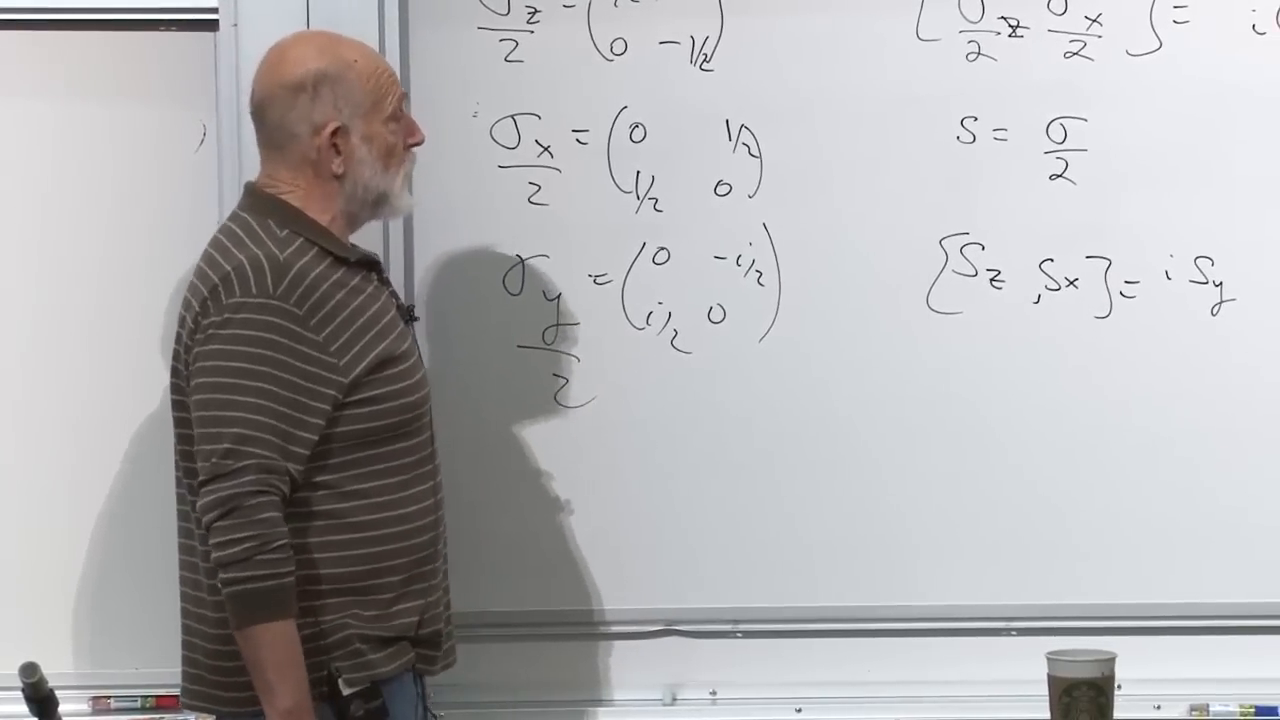
\includegraphics[width=0.9\linewidth]{lecture_04_frame_02.png}
\caption{في وحدات يكون فيها \(\hbar=1\)، تكون أنصاف مصفوفات باولي مؤثرات الزخم الزاوي للّفّ المغزلي نصفيّ وتحقق \([S_z,S_x]=iS_y\).}
\lectureframe{00:55:41}
\end{figure}

معادلتا القيم الذاتية لـ \(S_z\) هما
\begin{equation}
S_z\lvert\pm\rangle
=\pm\frac{\hbar}{2}\lvert\pm\rangle.
\end{equation}
وبصورة مكافئة، يكون عدد الكم المغناطيسي عديم الأبعاد
\begin{equation}
m_{s}=\pm\frac12,
\qquad
S_{z}\lvert m_{s}\rangle
=m_{s}\hbar\,\lvert m_{s}\rangle.
\end{equation}
وتغيّر مؤثرات الرفع والخفض للزخم الزاوي قيمة \(m\) بمقادير صحيحة، لكن هذا لا يقتضي أن يمر كل سلم عبر الصفر. فالمتعددات الصحيحة تضم قيمًا صحيحة لـ \(m\)، في حين تضم المتعددات نصف الصحيحة قيمًا نصف صحيحة. وبالنسبة إلى اللفّ المغزلي نصفيّ، لا يضم السلم إلا العضوين \(m_s=+1/2\) و\(m_s=-1/2\).

تشكل هاتان الحالتان ثنائية اللفّ المغزلي نصفيّ. ومن بين الجسيمات التي توصف بمثل هذه المتعددات ذات اللفّ المغزلي نصف الصحيح الإلكترونات والميونات والنيوترينوات والكواركات.

\section{الزخم الزاوي المداري واللفّ المغزلي}

لدينا الآن نوعان من الزخم الزاوي. فالزخم الزاوي المداري يصف الحركة بالنسبة إلى مبدأ إحداثي،
\begin{equation}
\mathbf L=\mathbf R\times\mathbf P,
\end{equation}
في حين أن \(\mathbf S\) هو اللفّ المغزلي الجوهري. ومجموعهما المتجهي هو الزخم الزاوي الكلي،
\begin{equation}
\mathbf J=\mathbf L+\mathbf S.
\end{equation}

\begin{classroomqa}
\lecturetimestamp{00:56:49}
\audiencequestion{إذا كان للنظام زخم زاوي كلي \(\mathbf J\)، فكيف يُحدَّد لفّه المغزلي \(\mathbf S\)؟}
\lecturerresponse{يُعطى عدد الكم المغزلي وعدد الكم المداري عادةً كلٌّ منهما على حدة. فإذا كان \(L=0\)، كان الزخم الزاوي كله لفًّا مغزليًا. وإلا لزمت القواعد الكمومية لجمع الزخوم الزاوية، وهي مؤجَّلة هنا.}
\end{classroomqa}

تنطبق قواعد الجمع على الزخم الزاوي المداري مضافًا إلى اللفّ المغزلي، وعلى لفّين مغزليين، أو على زخمين زاويين مداريين. وللنظام المركب قيمه المسموح بها الخاصة للزخم الزاوي الكلي، لكننا لا نحتاج إلى تلك القواعد بعد.

\begin{classroomqa}
\lecturetimestamp{00:58:18}
\audiencequestion{ما الدليل التجريبي الذي أدى إلى إدخال اللفّ المغزلي؟}
\lecturerresponse{قدّم التحليل الطيفي دليلًا، لكن الجدول الدوري يوفّر دافعًا واضحًا على نحو خاص: فبنيته القشرية تقتضي أن تمتلك الإلكترونات خاصية إضافية ثنائية القيم.}
\end{classroomqa}

\section{الانحلال الشبيه بالهيدروجين وعدّ الأغلفة}

بالنسبة إلى الزخم الزاوي المداري، فإن معادلة القيمة الذاتية لـ \(L^{2}\) هي
\begin{equation}
L^{2}\lvert\ell,m\rangle
=\hbar^{2}\ell(\ell+1)\lvert\ell,m\rangle,
\end{equation}
ولقيمة ثابتة من \(\ell\) يوجد
\begin{equation}
2\ell+1
\end{equation}
من الحالات المغناطيسية، الموافقة لـ \(m=-\ell,-\ell+1,\ldots,\ell\).

لمسألة كولوم المثالية غير النسبية انحلال إضافي. وطاقات حالاتها المقيدة سالبة وتقترب من الصفر من الأسفل، ولكن الذي يهم في العد هو تحاذي المستويات فحسب. فالمستوى الأول \(\ell=1\) يتحاذى مع المستوى التالي \(\ell=0\)؛ ويلتحق المستوى الأول \(\ell=2\) بالغلاف الرئيسي التالي؛ ويستمر النمط على هذا المنوال.\footnote{\texttt{lecture\_04\_frame\_03.png}، عند \(01{:}02{:}01\)؛ ويُذكر التحاذي الكامل للأغلفة الرئيسية من \(01{:}02{:}33\) إلى \(01{:}04{:}10\).}

\begin{figure}[htbp]
\centering
\begin{tikzpicture}[x=1.55cm,y=1.0cm]
\draw[->] (-0.65,0) -- (-0.65,4.35);
\draw[->] (-0.85,0) -- (4.75,0);
\node at (-0.95,4.08) {\(E\)};
\node at (4.55,-0.28) {\(\ell\)};
\node at (0,-0.30) {\(0\)};
\node at (2,-0.30) {\(1\)};
\node at (4,-0.30) {\(2\)};

\draw (-0.20,0.75) -- (0.20,0.75);

\draw (-0.20,2.00) -- (0.20,2.00);
\foreach \dx in {-0.18,0,0.18}
  \draw (2+\dx-0.06,2.00) -- (2+\dx+0.06,2.00);

\draw (-0.20,3.15) -- (0.20,3.15);
\foreach \dx in {-0.18,0,0.18}
  \draw (2+\dx-0.06,3.15) -- (2+\dx+0.06,3.15);
\foreach \dx in {-0.32,-0.16,0,0.16,0.32}
  \draw (4+\dx-0.05,3.15) -- (4+\dx+0.05,3.15);

\node[anchor=west] at (0.35,0.75) {\(n=1\)};
\node[anchor=west] at (2.35,2.00) {\(n=2\)};
\node[anchor=west] at (4.40,3.15) {\(n=3\)};
\end{tikzpicture}
\caption{تجمع الأغلفة الكولومية المثالية الثلاثة الأولى متعددات مدارية ذات الطاقة الرئيسية نفسها: حالة واحدة في الغلاف الأول، و\(1+3\) في الثاني، و\(1+3+5\) في الثالث.}
\lectureframe{01:02:01}
\end{figure}

في الغلاف الرئيسي \(n\)، تكون القيم المدارية المسموح بها هي\footnote{يعيد هذا المجال الموجز لـ \(\ell\) والمجموع أدناه بناء تحاذيات المستويات والأعداد \(1,4,9,16,\ldots\) المذكورة من \(01{:}02{:}33\) إلى \(01{:}04{:}10\). ويظهر بدء رسم الطيف في \texttt{lecture\_04\_frame\_03.png} عند \(01{:}02{:}01\).}
\[
\ell=0,1,\ldots,n-1.
\]
ولذلك فإن عدد الحالات المكانية هو
\begin{equation}
\sum_{\ell=0}^{n-1}(2\ell+1)=n^{2},
\end{equation}
فتنتج المتتالية
\begin{equation}
1,\ 4,\ 9,\ 16,\ldots .
\end{equation}
وهذا عدّ مداري فقط. فكل حالة مكانية تسمح بقيمتين لللفّ المغزلي، ولذلك تكون المجاميع المثالية المناظرة
\begin{equation}
2,\ 8,\ 18,\ 32,\ldots=2n^{2}.
\end{equation}

\section{الاستبعاد وخاصية الإلكترون ثنائية القيم}

لنبدأ بالهيليوم في تقريب الإلكترونات المستقلة. فنواته تحمل ضعف شحنة البروتون، مما يعيد تحجيم المستويات الشبيهة بالهيدروجين ويجذب الإلكترونات إلى الداخل. وإذا تجاهلنا مؤقتًا تآثرات الإلكترون--الإلكترون، فيمكن لإلكترونين أن يشغلا المدار المكاني الأدنى ويعطيا تقريبًا أوليًا معقولًا للحالة الأرضية للهيليوم.

ولِمَ لا نضع إلكترونًا ثالثًا هناك أيضًا؟ فذلك من شأنه أن يخفض طاقته المدارية، لكن هذا لا يحدث. والقيد هو مبدأ استبعاد باولي: فلا يجوز لإلكترونين أن يشغلا الحالة الكاملة نفسها لجسيم واحد. وسيكون من المضلل تسمية ذلك قوة تنافر عادية. إنه قيد على الحالة الكمومية المسموح بها.

توجد هنا مفارقة ظاهرية. فإلكترونا الهيليوم يشتركان فعلًا في المدار المكاني نفسه. والحل هو أن حالة الإلكترون الكاملة تتضمن أكثر من الدالة الموجية المدارية. فهي تتضمن أيضًا درجة حرية ثنائية القيم. ولنسمِّ القيمتين أعلى وأسفل. فيمكن أن يكون أحد الإلكترونين في المدار الأدنى بلفٍّ مغزلي إلى أعلى والآخر بلفٍّ مغزلي إلى أسفل؛ فتتطابق حالتهما المكانية، لكن حالتيهما الكموميتين الكاملتين لا تتطابقان.

عند هذه النقطة يبدأ العدّ بالتقدم نحو الليثيوم ثم يتراجع. ويكشف هذا الرجوع لماذا يكون كلٌّ من الاستبعاد واللفّ المغزلي ضروريًا. تخيّل قاعدة استبعاد بلا أي لفّ مغزلي على الإطلاق. عندئذ لا يستطيع شغل أدنى حالة مكانية إلا إلكترون واحد. وسيضطر إلكترون ثانٍ إلى الدخول في إحدى الحالات المكانية الأربع في الغلاف الرئيسي التالي، فينتج عن ذلك عدة احتمالات حيث تكون الحالة الأرضية المرصودة للهيليوم فريدة. وتلك الصيغة من الاستبعاد من دون لفّ مغزلي خاطئة.

أعِد القيمتين لللفّ المغزلي. يملأ إلكترونان المدار الأدنى بلفّين مغزليين متعاكسين. ويجب على إلكترون ثالث، كما في الليثيوم المتعادل، أن يدخل الغلاف الرئيسي التالي. ففي ذلك الغلاف حالة مكانية واحدة ذات \(\ell=0\) وثلاث حالات مكانية ذات \(\ell=1\). وقبل احتساب اللفّ المغزلي توجد أربع إمكانات.

\begin{classroomqa}
\lecturetimestamp{01:14:58}
\audiencequestion{كيف تعطي حالات \(s\) و\(p\) ثماني إمكانات في أول غلاف مُثار؟}
\lecturerresponse{توجد حالة مكانية واحدة ذات \(\ell=0\) وثلاث حالات ذات \(\ell=1\)، فيكون المجموع أربع حالات مكانية. وتقبل كل واحدة منها قيمتين لللفّ المغزلي، لذا يكون المجموع \(2(1+3)=8\).}
\end{classroomqa}

هذا هو العدّ البسيط الكامن وراء العناصر الثمانية في الصف الثاني من الجدول الدوري. وهو تبسيط مثالي مقصود عمدًا: فالمناقشة اللاحقة ستوضح أن تآثرات الإلكترون--الإلكترون تفسد سريعًا صورة الأغلفة المستقلة الشبيهة بالهيدروجين.

يمكن أيضًا اختبار الخاصية ذات القيمتين بوصفها عزمًا زاويًا. فلفّ الإلكترون الذاتي يصاحبه عزم مغناطيسي، ولذلك يمنح المجال المغناطيسي إسقاطي لفّه طاقتين مختلفتين. والمستوى الذي كان منحلًّا عند انعدام المجال ينشطر إلى مستويين، تمامًا كما هو متوقع لعزم مغناطيسي صغير موازٍ للمجال أو معاكس له. ويختبر هذا الانشطار ما إذا كانت درجة الحرية ذات القيمتين المضافة تتصرف كعزم زاوي لا كوسم ثنائي اعتباطي.

\section{الفوتونات والإلكترونات وحدود تصور الأغلفة}

لا تخضع جميع الجسيمات لقاعدة الإشغال نفسها. فقد يمكن لعدد كبير من الفوتونات أن يشغل النمط الكهرومغناطيسي نفسه؛ ويمكن فهم الموجة الضوئية الكلاسيكية على أنها حالة تحتوي عددًا كبيرًا من الفوتونات في ذلك النمط. أما الإلكترونات فتسلك على نحو مختلف: إذ يمنعها مبدأ الاستبعاد من التكدس في حالة كمومية كاملة واحدة. وهذا التباين هو ما يحفز التمييز بين نوعَي إحصاء الجسيمات.

\begin{classroomqa}
\lecturetimestamp{01:20:28}
\audiencequestion{ماذا يحدث لسيل حر من الإلكترونات بدلًا من إلكترونات مرتبطة في الذرات؟}
\lecturerresponse{تظل قاعدة الاستبعاد منطبقة: لا يمكن لجميع الإلكترونات أن تشغل حالة كمومية واحدة. ويمكن لليزر أن يضع كثيرًا من الفوتونات في النمط نفسه، لكن لا يمكن إعداد سيل إلكتروني على هذا النحو.}
\end{classroomqa}

هذا القيد خاصية للإلكترونات، وليس خصوصيةً للارتباط الذري.

\begin{classroomqa}
\lecturetimestamp{01:21:12}
\audiencequestion{هل العزم الزاوي المداري هو على وجه التحديد دوران حول نواة؟}
\lecturerresponse{يُعرَّف العزم الزاوي بالنسبة إلى أصل مختار. فالنواة هي الأصل الطبيعي في الذرة، بينما يكون للجسيم الحر عزم زاوي \(\mathbf R\times\mathbf P\) بالنسبة إلى أي أصل يُختار.}
\end{classroomqa}

كل مناقشة للدوران تختار نقطةً يُؤخذ الدوران حولها. وتوفر الذرة مركزًا طبيعيًا لأن نواتها هي مركز الجهد المركزي تقريبًا. وفي الفضاء الحر لا يكون أي أصل مفضلًا، مع أن العزم الزاوي يظل قابلًا للحساب بالنسبة إلى أي أصل مختار.

\begin{classroomqa}
\lecturetimestamp{01:22:34}
\audiencequestion{لماذا يحتوي الجدول الدوري على صفوف متكررة من ثمانية عناصر ثم صفوف متكررة من ثمانية عشر عنصرًا؟}
\lecturerresponse{إن تصور الأغلفة البسيط القائم على الإلكترونات المستقلة لا يفسر النمط الكامل. فهو ينهار سريعًا لأنه يهمل التآثرات بين الإلكترونات.}
\end{classroomqa}

في الذرة الكبيرة، تتآثر الإلكترونات الخارجية مع سحابة إلكترونية داخلية كبيرة، وكذلك مع النواة. ولم يعد من المعقول معاملة كل إلكترون كما لو كان يتحرك استقلالًا في مجال كولوم غير محجوب.

\begin{classroomqa}
\lecturetimestamp{01:23:33}
\audiencequestion{لماذا لا تزداد الذرات حجمًا زيادة هائلة مع إضافة مزيد من الإلكترونات؟}
\lecturerresponse{إن إضافة إلكترونات تعني أيضًا إضافة بروتونات إلى النواة. فالشحنة النووية المتزايدة تجذب الإلكترونات الداخلية إلى الداخل، بينما تحجب تلك الإلكترونات الداخلية تأثير النواة. وفي هذا التصور البسيط، يتحرك إلكترون تكافؤ خارجي عندئذٍ تحت تأثير شحنة فعالة تقارب الواحد.}
\end{classroomqa}

تؤدي زيادة الشحنة النووية إلى انكماش السحابة الداخلية. وبالنسبة إلى ذرة لها إلكترون تكافؤ خارجي واحد، يكاد تأثير النواة والإلكترونات الداخلية أن يتعادل عند المسافات الكبيرة، فيبقى إلكترون التكافؤ في مجال يشبه تقريبًا مجال شحنة موجبة وحدية. لذلك لا تنمو الأحجام الذرية ببساطة بنسبة طردية مع عدد الإلكترونات.

\begin{classroomqa}
\lecturetimestamp{01:24:49}
\audiencequestion{هل التنافر الكهربائي هو السبب في بقاء الذرات المتجاورة متباعدة؟}
\lecturerresponse{ليس بمفرده. فاستبعاد باولي يولد تنافرًا فعالًا مهمًا عندما تتراكب السحب الإلكترونية، وهو بالنسبة إلى كثير من الذرات السبب الغالب في مقاومتها لمزيد من التراكب.}
\end{classroomqa}

تنافر باولي نتيجة فعالة للاستبعاد، وليس قانون قوة إضافيًا.

\begin{classroomqa}
\lecturetimestamp{01:25:23}
\audiencequestion{هل مبدأ الاستبعاد مسلَّمة منفصلة؟}
\lecturerresponse{في ميكانيكا الكم غير النسبية يُفرَض بوصفه مسلَّمة. أما في نظرية الكم النسبية، فإن ارتباط اللف--الإحصاء يمنحه أساسًا أعمق.}
\end{classroomqa}

\section{الجسيمات المتماثلة في الميكانيكا الكلاسيكية وميكانيكا الكم}

قبل صياغة تلك المسلَّمة، تأمل كيف تُعَدّ الجسيمات المتماثلة في الميكانيكا الكلاسيكية. ضع جسيمين من النوع نفسه في مجموعة من الصناديق. فإذا كانت الجسيمات تحمل سرًا أسماءً ---Harry and Sally---، فإن وجود Harry في الصندوق الأول وSally في الثاني يبدو مختلفًا عن وجود Sally في الأول وHarry في الثاني.

تسمح الميكانيكا الكلاسيكية بتلك الصورة حتى عندما تكون العلامات خافتة إلى حد يتعذر كشفها. ويمكن تخيل علامة ضعيفة على نحو اعتباطي على كل جسيم، ومع ذلك يُنظر إلى مساريهما على أنهما متميزان. وفي الميكانيكا الإحصائية الكلاسيكية، يُختار عادةً عدم عدّ تبديلات الجسيمات المتماثلة تهيئات جديدة. ولـ \(N\) من الجسيمات، تعطي هذه الاتفاقية العامل المألوف \(1/N!\).

ميكانيكا الكم أشد صرامة. فالجسيمات المتماثلة لا تحمل وسومًا فردية خفية يمكن تتبعها من حيث المبدأ. وإلكترونان قابلان للتبادل بوصفهما إلكترونين. أما مبادلة إلكترون بفوتون فتنتج ترتيبًا مختلفًا فيزيائيًا لأنهما من نوعين مختلفين، لكن تبديل خانتي الإلكترونين لا يمكن أن يكشف أيّهما كان أيّهما بالفعل.

لحالة الجسيم الواحد دالة موجية
\[
\psi(x)=\langle x\vert\psi\rangle.
\]
وبالنسبة إلى جسيمين، تكون الحالة دالة في متغيري موضع،
\begin{equation}
\psi(x_{1},x_{2}).
\end{equation}
وتدل المؤشرات السفلى على الخانتين في الوصف، لا على اتجاهين مكانيين. ويعطي مربع مقدارها المطلق كثافة الاحتمال المشتركة للموضع.

\section{مؤثر التبادل ومسلَّمة الإحصاء}

بدّل خانتي الجسيمين:
\begin{equation}
\psi(x_{1},x_{2})\longmapsto\psi(x_{2},x_{1}).
\end{equation}
وباتباع الترميز المستخدم في هذه المناقشة، لنرمز إلى مؤثر التبادل بـ \(S\). وهنا يرمز \(S\) إلى التبادل، لا إلى متجه اللف \(\mathbf S\). ويكون فعله
\begin{equation}
(S\psi)(x_{1},x_{2})=\psi(x_{2},x_{1}).
\end{equation}
ولا يلزم أن تكون الدالة العامة في متغيرين متناظرة، لذا يمكن لهذه العملية أن تنتج دالة موجية مختلفة.

إن إجراء التبادل مرتين يعيد الترتيب الأصلي:
\begin{equation}
S^{2}=I.
\end{equation}
والتبادل قابل للعكس ويحفظ الجداءات الداخلية، لذا يمثَّل بمؤثر وحيدي. فإذا كانت \(\psi\) متجهة ذاتية لـ \(S\) بالقيمة الذاتية \(\lambda\)، فإن
\[
S^{2}\psi=\lambda^{2}\psi=\psi,
\]
ومن ثم
\begin{equation}
\lambda=\pm1.
\end{equation}

تحدد هذه النتيجة فضاءين ذاتيين للتبادل، لكنها لا تقول إن كل دالة موجية اعتباطية لجسيمين هي أصلًا متجهة ذاتية لـ \(S\). ويمكن فصل أي دالة من هذا النوع إلى جزأيها،\footnote{هذا التفكيك توضيح جبري تحريري للفضاءين الذاتيين اللذين يقتضيهما \(S^{2}=I\). وتذكر الحجة الواردة القيمتين الذاتيتين ثم تُدخل بعد ذلك مبدأ الإحصاء الإضافي.}
\begin{equation}
\psi_{\pm}=\frac12(I\pm S)\psi,
\end{equation}
وهما يحققان
\begin{equation}
S\psi_{\pm}=\pm\psi_{\pm}.
\end{equation}
ومن ثم
\begin{align}
\psi_{+}(x_{2},x_{1})&=\psi_{+}(x_{1},x_{2}),\\
\psi_{-}(x_{2},x_{1})&=-\psi_{-}(x_{1},x_{2}).
\end{align}

والآن يأتي مبدأ إضافي، وليس نتيجةً لـ \(S^{2}=I\) وحده. فبالنسبة إلى الجسيمات المتماثلة من أي نوع بعينه، تقع الحالات المسموح بها كلها ضمن أحد قطاعي التبادل هذين: فتبادل زوج منها إما أن يعيد الدالة الموجية نفسها دائمًا، وإما أن يعيد سالبها دائمًا. والقطاع \(+1\) متناظر، والقطاع \(-1\) مضاد التناظر. وأما التفسير الفيزيائي لهذين الاحتمالين بوصفهما نوعَي إحصاء الجسيمات، فهو الخطوة التالية، ويُترك للمناقشة الآتية.
